\documentclass[a4paper,12pt]{report}
\usepackage[utf8]{inputenc} % style d'écriture
\usepackage[T1]{fontenc}      % package
\usepackage[francais]{babel}  % package pour langue française
\usepackage[a4paper]{geometry} % definition des marges
\usepackage[pdftex]{graphicx} % definition d'image
\usepackage{fancyhdr} % haut de page
\usepackage{float}
\usepackage{tcolorbox,listings}
\usepackage{caption}
\addtocounter{tocdepth}{3}
\setcounter{secnumdepth}{3}
\usepackage{color}


\lstset{
  aboveskip=5mm,
  belowskip=-2mm,
  basicstyle=\footnotesize,
  breakatwhitespace=false,
  breaklines=true,
  captionpos=b,
  commentstyle=\color{red},
  deletekeywords={...},
  escapeinside={\%*}{*)},
  extendedchars=true,
  framexleftmargin=16pt,
  framextopmargin=3pt,
  framexbottommargin=6pt,
  frame=tb,
  keepspaces=true,
  keywordstyle=\color{blue},
  language=VHDL,
  literate=
  {²}{{\textsuperscript{2}}}1
  {⁴}{{\textsuperscript{4}}}1
  {⁶}{{\textsuperscript{6}}}1
  {⁸}{{\textsuperscript{8}}}1
  {€}{{\euro{}}}1
  {é}{{\'e}}1
  {è}{{\`{e}}}1
  {ê}{{\^{e}}}1
  {ë}{{\"{e}}}1
  {É}{{\'{E}}}1
  {Ê}{{\^{E}}}1
  {û}{{\^{u}}}1
  {ù}{{\`{u}}}1
  {â}{{\^{a}}}1
  {à}{{\`{a}}}1
  {á}{{\'{a}}}1
  {ã}{{\~{a}}}1
  {Á}{{\'{A}}}1
  {Â}{{\^{A}}}1
  {Ã}{{\~{A}}}1
  {ç}{{\c{c}}}1
  {Ç}{{\c{C}}}1
  {õ}{{\~{o}}}1
  {ó}{{\'{o}}}1
  {ô}{{\^{o}}}1
  {Õ}{{\~{O}}}1
  {Ó}{{\'{O}}}1
  {Ô}{{\^{O}}}1
  {î}{{\^{i}}}1
  {Î}{{\^{I}}}1
  {í}{{\'{i}}}1
  {Í}{{\~{Í}}}1,
  morekeywords={*,...},
  numbers=left,
  numbersep=10pt,
  numberstyle=\tiny\color{black},
  rulecolor=\color{black},
  showspaces=false,
  showstringspaces=false,
  showtabs=false,
  stepnumber=1,
  stringstyle=\color{gray},
  tabsize=4,
  title=\lstname,
}

%\captionsetup[figure]{labelformat=empty}
\renewcommand{\thesection}{\Roman{section}}

\begin{document}
   \begin{titlepage}
    
    \newcommand{\HRule}{\rule{\linewidth}{0.5mm}} % Defines a new command for the horizontal lines, change thickness here
    
    \center % Center everything on the page
     
    %----------------------------------------------------------------------------------------
    %	HEADING SECTIONS
    %----------------------------------------------------------------------------------------
    
    \textsc{\LARGE Université de Bretagne Occidentale}\\[1.5cm] % Name of your university/college
		\textsc{\Large Master 2 Informatique}\\[0.5cm] % Major heading such as course name
		\textsc{\Large Département Informatique}\\[1.5cm] % Major heading such as course name
		{\large 2020/2021}\\[1.5cm] % Date, change the \today to a set date if you want to be precise
		
    \textsc{\large Système On-Chip}\\[1cm] % Minor heading such as course title
    
    %----------------------------------------------------------------------------------------
    %	TITLE SECTION
    %----------------------------------------------------------------------------------------
    
   \HRule \\[0.4cm]
    { \huge \bfseries Détection de dépassement de temps d'exécution}\\[0.2cm] % Title of your document
    \HRule \\[1cm]
     
    %----------------------------------------------------------------------------------------
    %	AUTHOR SECTION
    %----------------------------------------------------------------------------------------
    
    \begin{minipage}{0.48\textwidth}
			\begin{flushleft} \large
				\emph{Auteur:}\\
					William \textsc{PENSEC} % Your name
			\end{flushleft}
    \end{minipage}
		~
		\begin{minipage}{0.48\textwidth}
			\begin{flushright} \large
				\emph{Auteur:}\\
					Timothé \textsc{LANNUZEL} % Your name
			\end{flushright}
    \end{minipage}\\[1.5cm]
    
    %----------------------------------------------------------------------------------------
    %	DATE SECTION
    %----------------------------------------------------------------------------------------
    
    {\today}\\[1.5cm] % Date, change the \today to a set date if you want to be precise
    
    %----------------------------------------------------------------------------------------
    %	LOGO SECTION
    %----------------------------------------------------------------------------------------
    
		\begin{minipage}{0.48\textwidth}
			\begin{flushleft} \large
				
\includegraphics[scale=0.8]{ubo_sc.png} % Include a department/university logo - this will require the graphicx package
			\end{flushleft}
    \end{minipage}
		~
    \begin{minipage}{0.48\textwidth}
			\begin{flushright} \large
				
\includegraphics[scale=0.5]{ubo.png} % Include a department/university logo - this will require the graphicx package
			\end{flushright}
    \end{minipage}
    
    %----------------------------------------------------------------------------------------
    
    \vfill % Fill the rest of the page with whitespace
    
    \end{titlepage}
		
	\pagestyle{fancy}
		\lhead{}
		\chead{William PENSEC \& Timothé LANNUZEL}
		\rhead{}
		\lfoot{}
		\cfoot{\thepage}
		\rfoot{}
		
	\newpage\renewcommand{\contentsname}{Sommaire}
	\tableofcontents

	\newpage
	\section{Introduction}
		\paragraph*{}
		L'objectif de ce projet est de concevoir en VHDL un moniteur de temps d'exécution de tâches sur un processeur. En effet, sur un système temps réel, il est très important que les contraintes de temps soient respectées afin d'éviter tout problèmes. Le composant doit suivre l'exécution de chaques tâches et envoyer un signal d'interruption au processeur si l'une d'entre elles dépasse son échéance. La capacité maximale d'une tâche s'appelle le Worst Case Execution Time (WCET). En connaissant cette valeur, on sait si le processeur peut gérer le système ou s'il est nécessaire de le changer pour quelque chose de plus performant.
		
	\section{Conception VHDL}
		\paragraph*{}
		Le projet s'est découpé en plusieurs étapes qui ont été de créer d'abord les différents modules qui composent le système puis de créer les fichiers de tests (testbench) de ces modules.
		La seconde étape est de regrouper ces modules afin de créer une IP sous Vivado qui pourra être utilisée ailleurs.
		Cette IP sera composée du CPU, d'une mémoire, de compteurs et d'un composant permettant la communication avec le CPU par l'AXI.
		
		\begin{figure}[H]
			\centering
				\includegraphics[scale=1]{schemagen.png}
				\caption{Architecture générale}
			\label{archi}
		\end{figure}
		
		\subsection{Chronomètre}
			\paragraph*{}
			L'image \ref{chrono}, à la page \pageref{chrono}, représente le fonctionnement de manière schématique du module chronomètre-décompteur. Le code de cette partie est disponible dans l'archive ou sinon voir le code \ref{chronoCode} à la page \pageref{chronoCode}.
			Le chronomètre est lié à une horloge sur front montant \texttt{rising\_edge(clk)}. Cela permet de contrôler les opérations un front sur deux pour aller un peu plus lentement.
			Autrement, il y a un port de démarrage/arrêt du chronomètre \texttt{startStop} qui permet comme son nom l'indique de démarrer ou stopper le module; mais également un port afin de mettre en pause et de reprendre le timer \texttt{suspendResume}. Nous avons inclu un port de chargement \texttt{load} et de reset \texttt{reset} permettant de charger la valeur d'initialisation (valeur qui correspond à la durée du timer par exemple <10> périodes d'horloge) ou au contraire de mettre à 0 le timer de la tâche en cours.
			
			Enfin, le dernier port qui est celui qui nous intéresse le plus est celui du \texttt{wcet}. Ce port est donc un tableau de 16 bits. C'est dans ce tableau que l'on va enregistrer la valeur du \texttt{Worst Case Execution Time} (\texttt{WCET}). C'est cette valeur qui sera chargée par le port load en mémoire et c'est cette valeur qui servira à décompter le temps avant d'envoyer si besoin l'interruption au processeur si le \texttt{WCET} arrive à 0 dans le timer.
			
			\begin{figure}[H]
				\centering
					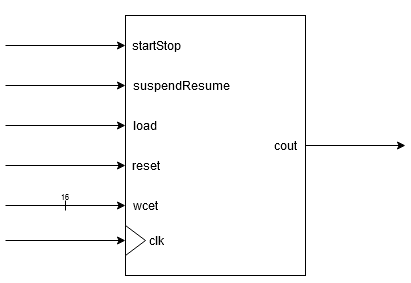
\includegraphics[scale=1]{chrono.png}
					\caption{Bloc chronomètre}
				\label{chrono}
			\end{figure}
			
			
		\subsection{TestBench Chronomètre}
			\paragraph*{}
			Le code du test bench est le code \ref{tbChronoCode} à la page \pageref{tbChronoCode}. Il s'articule de la manière suivante : tout d'abord comme d'habitude nous appellons le component à qui il fait référence, c'est à dire le chronomètre. Puis, on crée les signaux nécessaires pour assigner des valeurs aux ports du composant. Ensuite dans l'architecture comportementale du composant test, on affecte des valeurs aux signaux. Nous avons décidé de faire une horloge avec une période de 1 ns afin d'avoir quelque chose de rapide. La valeur \texttt{startStop\_ch} est initialisée à 0 et passe à 1 après 5 ns c'est à dire que le chronomètre ne démarrera qu'après 5 ns d'exécution de programme, cette valeur a été mise seulement dans un but de test mais en soit doit être initialisée à 1 lors de la création du chronomètre. La valeur \texttt{load\_ch} correspondant au chargement du \texttt{WCET} en mémoire; il est initialisé à 1, c'est à dire qu'on charge en mémoire la donnée dès qu'elle est disponible puis on passe cette valeur à 0 car on désire arrêter la mise en mémoire de la valeur afin de passer à la décrémentation. La valeur du \texttt{reset} est laissé à 0 car nous n'en avons pas besoin du tout mais si on passe cette valeur à 1 alors la donnée est mise à 0 comme convenu ! Enfin, la valeur du \texttt{wcet\_ch} est initialisée à 7.
			
		\subsection{Moniteur de tâches}
			\paragraph*{}
	
	
		\subsection{TestBench Moniteur de tâches}
			\paragraph*{}
			
			
	\section{Résultats}
		%\paragraph*{}
		
		\subsection{Chronomètre}
			\paragraph*{}
			
			\begin{figure}[H]
				\centering
					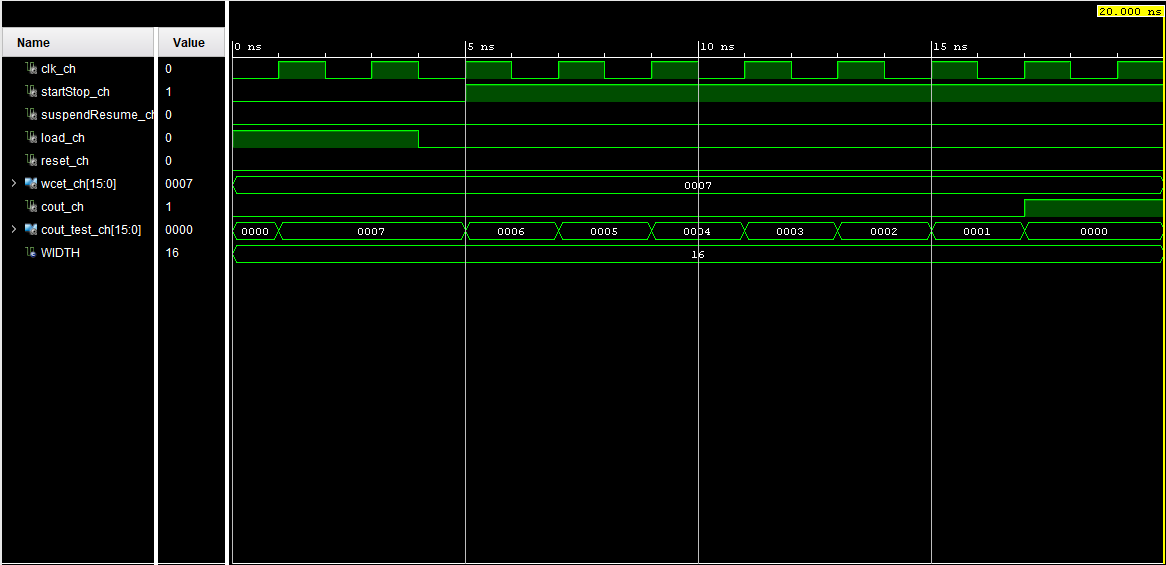
\includegraphics[scale=0.5]{chrono_tb.png}
					\caption{Testbench Chronomètre}
				\label{chronoTB}
			\end{figure}
			
		%\subsection{}
			%\paragraph*{}
	
	
	\section{Code}
		\subsection{Chronomètre}
			\lstinputlisting[caption={Chronomètre}, label={chronoCode}]{"code/chronometer.vhd"}
		
		\subsection{TestBench Chronomètre}
			\lstinputlisting[caption={TestBench Chronomètre}, label={tbChronoCode}]{"code/chronometer_tb.vhd"}
			
		\subsection{Moniteur de tâches}
		
			
		\subsection{TestBench Moniteur de tâches}
		
		
	\section{Continuité du projet}
		\paragraph*{}
			
			
	\clearpage
\end{document}